
\subsection{Data qubit displacement}
The proposal \cite{OGorman2016} as described in section \ref{sec:PhysicalImplementation} utilises two distinct qubit arrays each of lattice constant $D$, separated by a distance $d$ perpendicular to the planes. To achieve reasonable interaction times compared to qubit decoherence times, distances $D = \SI{400}{\nano\metre}$ and $d = \SI{40}{\nano\metre}$ have been chosen for simulation.

It is may prove unrealistic, however, to expect to be able to deterministically place qubits with \si{\nano\metre} precision in a scalable manner. Resolutions of \SI{10}{\nano\metre} can be achieved using e-beam lithography \cite{Vieu2000a} or nanostencil masks \cite{Weis2008}, combined with single-ion implantation techniques \cite{Jamieson2005}. STM patterning techniques offer atomic precision of dopants in Si \cite{Schofield2003} but a method of maintaining this precision over an array several \si{\micro\metre} across remains elusive. 

To consider in detail the effect of these displacements, we generated uniformly random offsets to the position of each data qubit within a pillbox of heigh and radius $R$, as illustrated in fig.\@ \ref{fig:pillbox}. This form of displacement is the same as used in the proposal \cite{OGorman2016} and was chosen as the displacement in the $x$--$y$ plane would be expected to be uniformly radial, and the implantation depth in the $z$-axis would be independent from this.

To illustrate the errors qubit displacement creates, consider a set of typical qubit displacements as illustrated in fig.\@ \ref{fig:qubitdisplacements}. These displacements give each data qubit a different distance $r$ at which it is closest to the probe qubit as it passes overhead, resulting in a different interaction strength. Hence the phase accumulated for each data qubit varies from the ideal $\tfrac{\pi}{2}$ by an independent amount. These errors are systematic in that the same phases are picked up for each parity measurement, unlike the probe jitter considered in section \ref{sec:jitter}.

We find that for these displacements, the case of even parity (no bit-flips) yields close to a $2\pi$ evolution with $99.968\%$ probability of successfully measuring $\ket{+}$, from the evolution shown in fig.\@ \ref{fig:displacementnoerrors}. However, on introducing bit-flip errors to each of the four data qubits, different phase accumulations are observed as in fig.\@ \ref{fig:displacementerrors}.


\begin{figure}
	%\centering
	\begin{minipage}[t]{0.515\linewidth}
		\begin{flushleft}
		\subfloat[]{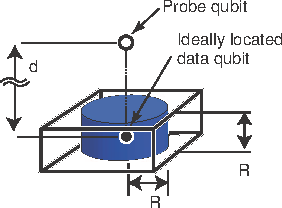
\includegraphics[width=0.6\linewidth]{../Figures/pillbox.pdf} \label{fig:pillbox}}\\
		\subfloat[]{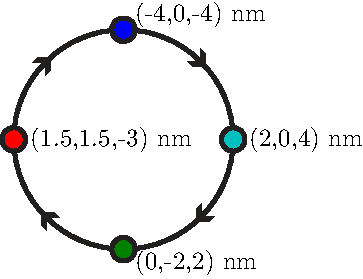
\includegraphics[width=0.7\linewidth]{../Figures/qubit_displacement_colours.pdf} \label{fig:qubitdisplacements}}
		\end{flushleft}
	\end{minipage}%
	\begin{minipage}[t]{0.485\linewidth}
	\subfloat[]{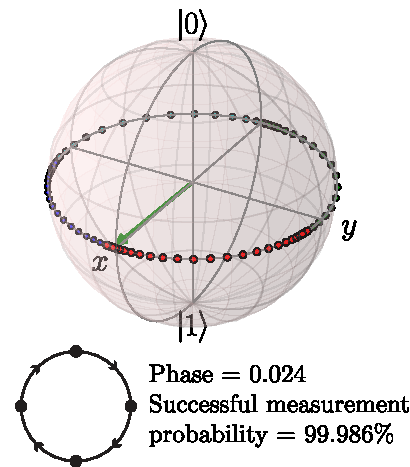
\includegraphics[width=\columnwidth]{../Figures/notwirl_noerror.pdf} \label{fig:displacementnoerrors}}
	\end{minipage}%
	
	\subfloat[]{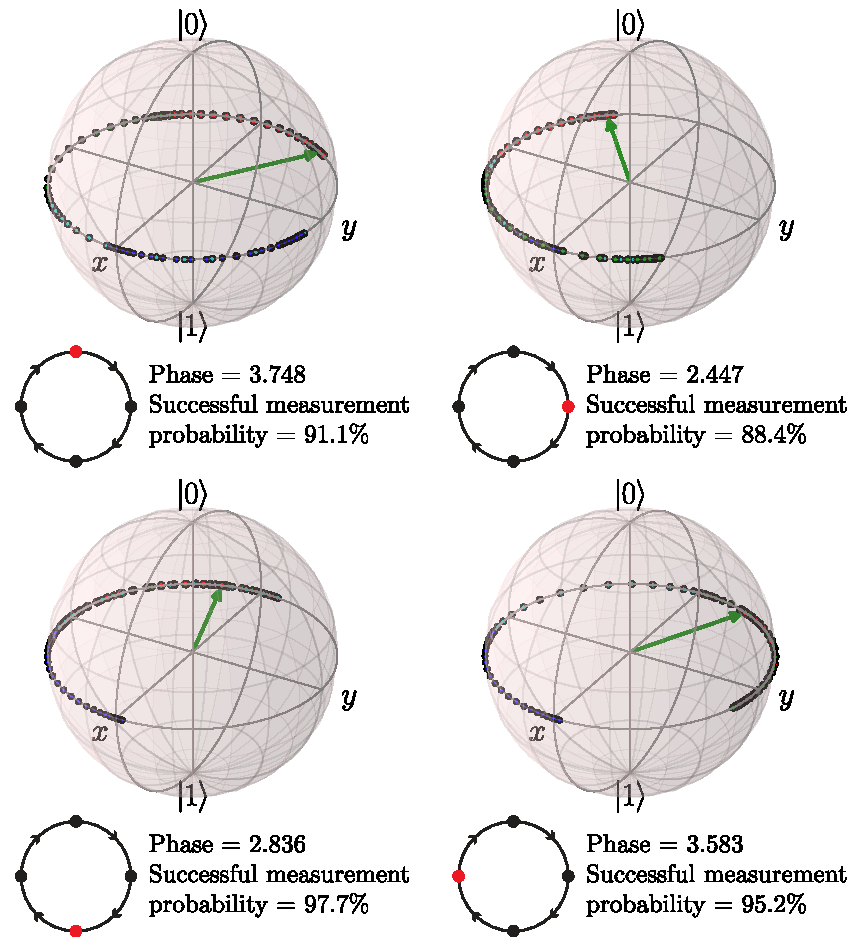
\includegraphics[width=1\columnwidth]{../Figures/notwirl_allerrors_portrait.pdf} \label{fig:displacementerrors}}
	
	\caption{Qubits displaced from the ideal lattice position give a phase contribution different to the ideal $\tfrac{\pi}{2}$ per qubit. (a) The pillbox region within which qubit displacements are randomly generated. Subfigure adapted from \cite{OGorman2016}. (b) The set of qubit displacements used to investigate the effects of displacement and twirling operations. (c) The phase accumulated and success probability for the displacements of (b) for even parity (no bit-flips). (c) The phase accumulated and success probability for each bit-flip error. Note the measurement success probability depends on which qubit is flipped, making the code susceptible to logical errors over repeated parity measurements. NOTE: change last subfigure to .pdf}
\end{figure}

%\begin{figure*}
%	\centering
%%	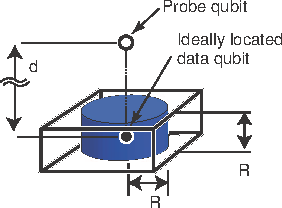
\includegraphics[width=\columnwidth]{../Figures/pillbox.pdf}
%	\subfloat[]{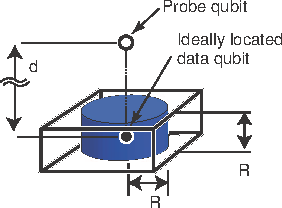
\includegraphics[width=0.7\columnwidth]{../Figures/pillbox.pdf} \label{fig:pillbox}}
%	\subfloat[]{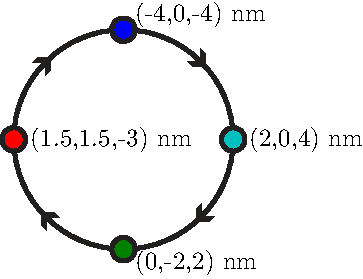
\includegraphics[width=0.7\columnwidth]{../Figures/qubit_displacement_colours.pdf} \label{fig:qubitdisplacements}}
%	\subfloat[]{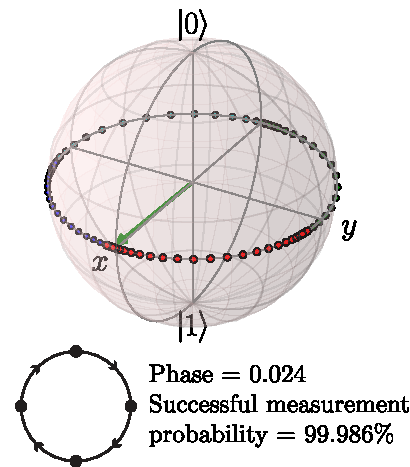
\includegraphics[width=0.5\columnwidth]{../Figures/notwirl_noerror.pdf} \label{fig:displacementnoerrors}}
%	
%	\subfloat[]{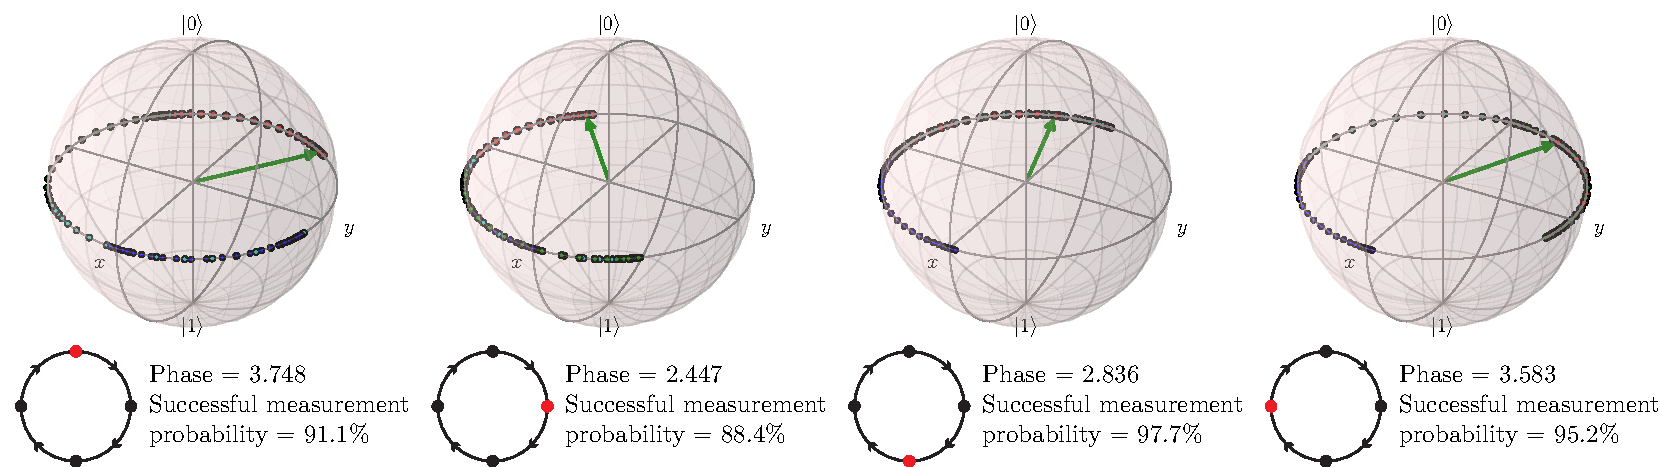
\includegraphics[width=2\columnwidth]{../Figures/notwirl_allerrors_landscape.pdf} \label{fig:displacementerrors}}
%	
%	\caption{Qubits displaced from the ideal lattice position give a phase contribution different to the ideal $\tfrac{\pi}{2}$ per qubit. (a) The pillbox region within which qubit displacements are randomly generated. Subfigure adapted from \cite{OGorman2016}. (b) The set of qubit displacements used to investigate the effects of displacement and twirling operations. (c) The phase accumulated and success probability for the displacements of (b) for even parity (no bit-flips). (c) The phase accumulated and success probability for each bit-flip error. Note the measurement success probability depends on which qubit is flipped, making the code susceptible to logical errors over repeated parity measurements. NOTE: change last subfigure to .pdf}
%\end{figure*}





